\documentclass{article} % Tạo một bản báo cáo
\usepackage[vietnamese]{babel}
\addto\captionsvietnamese{% Replace "Contents" with "Mục Lục"
  \renewcommand{\contentsname}%
    {MỤC LỤC}%
}
\usepackage[utf8]{inputenc}
\usepackage[T5]{fontenc} %Để sử dụng tiếng việt
\usepackage[fontsize=13pt]{scrextend} %set font size
\usepackage[paperheight=29.7cm, paperwidth=21cm, right=2cm, left=3cm, top=2cm, bottom=2.5cm]{geometry} %Chuẩn A4, căn lề phải, trái, trên, dưới
\usepackage{mathptmx} %Time new roman
\usepackage{graphicx} %Thư viện chèn ảnh
\usepackage{float} %set vị trí chèn ảnh
\usepackage{tikz} %thư viện tạo khung bìa
\usetikzlibrary{calc} %Thư viện tikz
\usepackage{indentfirst} % Thư viện thụt đầu dòng
\renewcommand{\baselinestretch}{1.2} % Giãn dòng 1.2
\setlength{\parskip}{6pt} % Spacing after
\setlength{\parindent}{1cm} % Set khoảng cách thụt đầu dòng mỗi đoạn
\usepackage{titlesec} % Thư viện để set up các kiểu chữ
\usepackage{hyperref} % Chuyển link khi click
\hypersetup{urlcolor=blue,linkcolor=black,citecolor=black,colorlinks=true}
\setcounter{secnumdepth}{4} % 4 Heading
\titlespacing*{\section}{0pt}{0pt}{30pt} % Heading 1
\titleformat*{\section}{\fontsize{16pt}{0pt}\selectfont \bfseries \centering}

\titlespacing*{\subsection}{0pt}{6pt}{0pt} % Heading 2
\titleformat*{\subsection}{\fontsize{14pt}{0pt}\selectfont \bfseries}

\titlespacing*{\subsubsection}{0pt}{6pt}{0pt} % Heading 3
\titleformat*{\subsubsection}{\fontsize{13pt}{0pt}\selectfont \bfseries \itshape}

\titlespacing*{\paragraph}{0pt}{0pt}{0pt} % Heading 4
\titleformat*{\paragraph}{\fontsize{13pt}{0pt}\selectfont \itshape}

\begin{document}
\begin{titlepage}

%Tạo khung
\begin{tikzpicture}[overlay,remember picture]
\draw [line width=3pt]
    ($ (current page.north west) + (3.0cm,-2.0cm) $)
    rectangle
    ($ (current page.south east) + (-2.0cm,2.5cm) $);
\draw [line width=0.5pt]
    ($ (current page.north west) + (3.1cm,-2.1cm) $)
    rectangle
    ($ (current page.south east) + (-2.1cm,2.6cm) $); 
\end{tikzpicture}
%Nội dung trong khung
\begin{center}
\vspace{-12pt}  TRƯỜNG ĐẠI HỌC SÀI GÒN \\
\textbf{\fontsize{14pt}{0pt}\selectfont KHOA CÔNG NGHỆ THÔNG TIN}
\vspace{0.4cm}
 \begin{figure}[H]
     \centering
     
\includegraphics[width=4cm,height=4cm]{images/SGU_LOGO.png}
 \end{figure}
\vspace{1.0cm}
\fontsize{16pt}{0pt}\selectfont BÁO CÁO ĐỒ ÁN\\
\vspace{12pt}
\textbf{\fontsize{18pt}{0pt}\selectfont PHÁT TRIỂN PHẦN MỀM MÃ NGUỒN MỞ}
\vspace{1.5cm}
\end{center}
\begin{center}
    \textbf{\fontsize{20pt}{0pt}\selectfont ĐỀ TÀI: PHÁT TRIỂN PHẦN MỀM TẢI VÀ CHUYỂN ĐỔI ĐỊNH DẠNG VIDEO YOUTUBE}
\vspace{1.5cm}
\begin{table}[H]
\centering
\begin{tabular}{l l}
    \fontsize{14pt}{0pt}\selectfont Sinh viên thực hiện:    & \fontsize{14pt}{0pt}\selectfont 3120410064 - Mai Ngọc Cảnh \vspace{6pt} \\ 
     &\fontsize{14pt}{0pt}\selectfont 3120410073 - Nguyễn Chí Công \vspace{6pt}\\
    \fontsize{14pt}{0pt}\selectfont Email liên hệ: & \fontsize{14pt}{0pt}\selectfont maicanh2002@gmail.com \vspace{50pt} \\
    \fontsize{14pt}{0pt}\selectfont Giảng viên hướng dẫn: & \fontsize{14pt}{0pt}\selectfont ThS. TỪ LÃNG PHIÊU
\end{tabular}
\end{table}
\vspace{2cm}
 \fontsize{14pt}{0pt}\selectfont Hồ Chí Minh, 4-2024
\end{center}
\end{titlepage}
\cleardoublepage

 % Tạo mục lục tự động
\addtocontents{toc}{\protect\thispagestyle{empty}}
\tableofcontents 
\thispagestyle{empty}
\cleardoublepage

\pagenumbering{arabic} % Đánh số thứ tự 1,2,3
\phantomsection %Tạo điểm cho href nhảy đến cho section*
\section*{GIỚI THIỆU DỰ ÁN}
\addcontentsline{toc}{section}{\numberline {}GIỚI THIỆU DỰ ÁN}
Trong một thế giới ngày càng trở nên số hóa, việc truy cập và chia sẻ nội dung video trực tuyến từ các platform như YouTube đã trở thành một phần không thể thiếu của cuộc sống hàng ngày của chúng ta. Tuy nhiên, đôi khi chúng ta muốn lưu trữ video từ YouTube vào thiết bị của mình hoặc chuyển đổi chúng sang các định dạng khác để phù hợp với các nhu cầu khác nhau. 

Trong dự án này nhóm 14 sẽ phát triển một phần mềm download và chuyển đổi định dạng video YouTube bằng ngôn ngữ lập trình Python. Phần mềm này sẽ cung cấp một giao diện đơn giản và dễ sử dụng cho người dùng, cho phép họ nhập URL của video YouTube mà họ muốn tải xuống và chuyển đổi. 

Mục tiêu của dự án này là giúp người dùng dễ dàng tải xuống và chuyển đổi video từ YouTube một cách thuận tiện và nhanh chóng. Bằng cách cung cấp một ứng dụng đơn giản nhưng mạnh mẽ, nhóm 14 hy vọng sẽ mang lại trải nghiệm tốt nhất cho người dùng khi xem lại những nội dung yêu thích ở mọi nơi.
\newpage
\phantomsection %Tạo điểm cho href nhảy đến cho section*
\section*{Chương 1. CƠ SỞ LÝ THUYẾT}
\addcontentsline{toc}{section}{\numberline {}Chương 1. CƠ SỞ LÝ THUYẾT}
\setcounter{section}{1}
\subsection{Ngôn ngữ Python}
\subsubsection{Python là gì?}
Python là một ngôn ngữ lập trình được sử dụng rộng rãi trong các ứng 
dụng web, phát triển phần mềm, khoa học dữ liệu và máy học (ML). 
Các nhà phát triển sử dụng Python vì nó hiệu quả, dễ học và có thể chạy 
trên nhiều nền tảng khác nhau. Phần mềm Python được tải xuống miễn 
phí, tích hợp tốt với tất cả các loại hệ thống và tăng tốc độ phát triển.
\subsubsection{Ưu điểm của Python}
Có một lý do mà các nhà phát triển chọn viết mã bằng Python. Nó có một số tính năng độc đáo giúp việc lập trình trở nên đơn giản hơn nhiều. Chúng ta hãy xem xét một số tính năng giúp làm việc với lợi thế của Python:
\begin{itemize}
    \item \textbf{Dễ đọc và dễ học:} Python là một ngôn ngữ đơn giản để đọc và học. Nó không có cú pháp phức tạp như các ngôn ngữ cấp cao khác như C hoặc C ++. Nhờ ít phức tạp hơn, Python cho phép bạn suy nghĩ rõ ràng hơn và tập trung vào việc xây dựng logic.
    \item \textbf{Giảm chi phí bảo trì:} Do tính đơn giản của nó, Python giúp bảo trì ứng dụng dễ dàng hơn và do đó, giảm chi phí liên quan, đây là một lợi thế lớn.
    \item \textbf{Khả năng ứng dụng rộng rãi:} Một tính năng thiết yếu khác của ngôn ngữ này là nó có thể áp dụng rộng rãi. Các kỹ sư, nhà khoa học và nhà toán học sử dụng rộng rãi nó.
    \item \textbf{Quản lý bộ nhớ:} Python có một thư viện rộng lớn với khả năng quản lý bộ nhớ, điều này làm cho nó nổi bật so với các ngôn ngữ lập trình khác. Nó bao gồm một heap riêng chứa tất cả các đối tượng và cấu trúc dữ liệu Python, một trình quản lý bộ nhớ tích hợp để duy trì heap riêng tư này.
    \item \textbf{Đơn giản và nhanh chóng:} Cộng đồng Python cung cấp hỗ trợ nhanh chóng và thiết thực cho người dùng cũng như khả năng thích ứng nhanh của mã. Một số chuyên gia thích đặt biệt danh cho Python là “ngôn ngữ sẵn sàng để chạy” vì nó chỉ yêu cầu mã đơn giản để được thực thi. Nâng cao và kiểm tra mã thoải mái hơn nhiều với Python.
    \item \textbf{Mã hóa không đồng bộ:} Mã hóa không đồng bộ sử dụng một vòng lặp sự kiện duy nhất để hoàn thành công việc trong những khoảng thời gian nhỏ. Python rất hữu ích để viết mã không đồng bộ vì nó dễ viết và dễ bảo trì. Nó không yêu cầu bất kỳ nội dung nghiên cứu phức tạp, bế tắc hoặc bất kỳ sự phức tạp nào khác.
    \item \textbf{Tích hợp với các ngôn ngữ khác:} Python có các thư viện như Cython và Jython, cho phép tích hợp với các ngôn ngữ khác như C, C ++ và Java để phát triển đa nền tảng. Đây là một trong những đặc quyền chính của Python vì không có ngôn ngữ nào là hoàn hảo và đôi khi sự phát triển đòi hỏi các chức năng ngôn ngữ đa dạng.
    \item \textbf{Tích hợp ứng dụng danh nghiệp:} Python là lựa chọn tốt nhất cho Tích hợp ứng dụng doanh nghiệp (EAI), cung cấp các tính năng kiểm soát quy trình đáng tin cậy và thực hiện các định dạng, giao thức dữ liệu internet. Hơn nữa, Python giúp người dùng xử lý các ngôn ngữ đánh dấu như XL, thực thi thông qua cùng một mã byte trên các hệ điều hành nâng cao và có thể được sử dụng như một ngôn ngữ kịch bản.
\end{itemize}
\subsubsection{Nhược điểm của Python}
Cùng với một số ưu điểm, Python có một số hạn chế trong các lĩnh vực hiệu suất và bảo mật. Sau đây là một số nhược điểm đáng kể của việc sử dụng Python:
\begin{itemize}
    \item \textbf{Tốc độ thực thi chậm:} Python là một ngôn ngữ thông dịch, có nghĩa là nó hoạt động với trình thông dịch, không phải với trình biên dịch. Do đó, nó thực thi tương đối chậm hơn C, C ++, Java và nhiều ngôn ngữ khác.
    \item \textbf{Tiêu thụ bộ nhớ lớn:} Các cấu trúc của Python đòi hỏi nhiều không gian bộ nhớ hơn. Ngôn ngữ này không thích hợp để sử dụng cho sự phát triển trong điều kiện bộ nhớ hạn chế.
    \item \textbf{Không thích hợp cho phát triển trò chơi và ứng dụng trên thiết bị di động:} Python chủ yếu được sử dụng trong phát triển máy tính để bàn và web phía máy chủ. Nó không được coi là lý tưởng để phát triển ứng dụng di động và phát triển trò chơi do tiêu tốn nhiều bộ nhớ hơn và tốc độ xử lý chậm so với các ngôn ngữ lập trình khác.
    \item \textbf{Hạn chế của nhà phát triển:} Một khi nhà phát triển đã quen với sự dễ dàng và đơn giản của ngôn ngữ này, họ sẽ khó sử dụng các ngôn ngữ khác.
    \item \textbf{Phát hiện lỗi trong mã:} Vì Python được thực thi thông qua trình thông dịch thay vì trình biên dịch, nên không thể phát hiện lỗi trong quá trình biên dịch và điều đó không tốt cho các nhà phát triển.
    \item \textbf{Quyền truy cập cơ sở dữ liệu:} Python được coi là không an toàn cao và có nguy cơ bảo mật. Có một số hạn chế khi sử dụng Python để truy cập cơ sở dữ liệu. So với các công nghệ phổ biến khác như JDBC và ODBC, lớp truy cập cơ sở dữ liệu Python hơi kém phát triển và sơ khai.
    \item \textbf{Hạn chế thiết kế:} Một trong những vấn đề quan trọng của Python là các hạn chế về thiết kế của nó.
    \item \textbf{Khó kiểm tra:} Vì nó là một ngôn ngữ dựa trên trình thông dịch, rất khó để chạy các bài kiểm tra trên mã được viết bằng Python. Tất cả các lỗi chỉ xuất hiện trong thời gian chạy, điều này khiến việc kiểm tra các đoạn mã được viết bằng Python rất khó khăn.
\end{itemize}

\subsection{Các thư viện chính trong dự án}
\subsubsection{tkinter} 
Tkinter là một thư viện giao diện người dùng (GUI) được tích hợp sẵn trong Python, cho phép bạn tạo ra các ứng dụng có giao diện đồ họa một cách dễ dàng.

Ưu điểm:
\begin{itemize}
    \item Dễ học và sử dụng: Tkinter được thiết kế để dễ học và sử dụng, đặc biệt là đối với những người mới bắt đầu với lập trình Python hoặc lập trình GUI.
    \item Hỗ trợ đa nền tảng: Tkinter hoạt động trên nhiều nền tảng, bao gồm Windows, macOS và Linux, giúp bạn xây dựng ứng dụng chạy trên nhiều hệ điều hành.
    \item Duy trì và phát triển: Tkinter đã tồn tại từ lâu và có cộng đồng lớn, điều này có nghĩa là bạn có thể tìm thấy nhiều tài liệu, ví dụ và hỗ trợ từ cộng đồng.
    \item Có sẵn các widget: Tkinter cung cấp một loạt các widget giao diện người dùng như nút, hộp văn bản, menu, danh sách, v.v., giúp bạn xây dựng giao diện người dùng phong phú và đa dạng.
\end{itemize}

\hspace{0.0em} Nhược điểm:

\begin{itemize}
    \item Giao diện trực quan đơn giản: Tkinter không cung cấp các tính năng hoạt động trực quan phức tạp như một số thư viện GUI khác như PyQt hoặc wxPython.
    \item Giao diện mặc định không thú vị: Giao diện mặc định của Tkinter có thể được coi là đơn giản và ít hấp dẫn hơn so với một số thư viện GUI khác.
    \item Hiệu suất: Tkinter không phải là thư viện GUI nhanh nhất, đặc biệt là khi xây dựng các ứng dụng lớn hoặc yêu cầu hiệu suất cao.
    \item Giới hạn của thiết kế giao diện: Tkinter có thể hạn chế trong việc tạo ra các giao diện người dùng phức tạp và hiện đại so với một số giải pháp GUI khác.
\end{itemize}
\subsubsection{customtkinter}
Thư viện customtkinter không phải là một thư viện chuẩn được tích hợp sẵn trong Python như Tkinter. Tuy nhiên, có thể đề cập đến một số thư viện được tạo ra bởi cộng đồng Python dưới tên customtkinter, nhằm mục đích cung cấp các tính năng mở rộng hoặc tùy chỉnh hơn cho việc phát triển ứng dụng GUI trong Python.

Ưu điểm:
\begin{itemize}
    \item Tích hợp các tính năng mở rộng: Một số phiên bản customtkinter có thể cung cấp các tính năng mở rộng hoặc tùy chỉnh cho Tkinter, như các widget hoặc chức năng phức tạp hơn so với những gì có sẵn trong Tkinter.
    \item Giúp tăng hiệu suất: Các phiên bản customtkinter có thể được tối ưu hóa để cải thiện hiệu suất hoặc cung cấp các tính năng hiệu suất cao hơn so với Tkinter.
    \item Tính linh hoạt cao: Một số phiên bản customtkinter có thể cung cấp tính linh hoạt cao hơn trong việc tạo giao diện người dùng, cho phép bạn tùy chỉnh giao diện một cách linh hoạt hơn.
    \item Cải thiện giao diện người dùng: Một số customtkinter có thể cung cấp các widget hoặc chức năng mở rộng giúp cải thiện giao diện người dùng của ứng dụng.
\end{itemize}
\hspace{0.0em} Nhược điểm:
\begin{itemize}
    \item Khả năng tương thích: Một số phiên bản customtkinter có thể không tương thích hoặc không ổn định như Tkinter, đặc biệt là khi sử dụng trong môi trường sản xuất.
    \item Tài liệu và hỗ trợ: Một số phiên bản customtkinter có thể thiếu tài liệu và hỗ trợ so với Tkinter, vì vậy việc học và sử dụng có thể khó khăn hơn.
    \item Khả năng bảo trì: Nếu không có sự hỗ trợ và bảo trì đầy đủ từ cộng đồng hoặc các nhà phát triển, các phiên bản customtkinter có thể trở nên lỗi thời hoặc không được bảo trì đúng cách.
\end{itemize}

\subsubsection{pytube}
Pytube là một thư viện Python mã nguồn mở được sử dụng để tải xuống video từ YouTube. Nó cung cấp một cách dễ dàng và linh hoạt để tương tác với API của YouTube và tải xuống video hoặc âm thanh từ các URL của video trên YouTube.

Ưu điểm:
\begin{itemize}
    \item Dễ sử dụng: Pytube được thiết kế để dễ sử dụng và cung cấp một API đơn giản và trực quan cho việc tải xuống video từ YouTube.
    \item Tích hợp sẵn trong Python: Pytube là một thư viện Python, nghĩa là không cần cài đặt bất kỳ phần mềm bên ngoài nào khác để sử dụng nó.
    \item Hỗ trợ đa nền tảng: Pytube hoạt động trên nhiều nền tảng, bao gồm Windows, macOS và Linux, cho phép bạn sử dụng nó trên nhiều hệ điều hành khác nhau.
    \item Tính linh hoạt: Pytube cung cấp các tùy chọn linh hoạt cho việc tải xuống video, bao gồm chất lượng video, định dạng file, và nhiều hơn nữa.
    \item Có sẵn các tính năng bổ sung: Pytube không chỉ hỗ trợ tải xuống video, mà còn hỗ trợ tải xuống âm thanh, lấy thông tin về video, và nhiều chức năng khác.
\end{itemize}
\hspace{0.0em} Nhược điểm:
\begin{itemize}
    \item Phụ thuộc vào API của YouTube: Pytube phụ thuộc vào API của YouTube để hoạt động, vì vậy nếu YouTube thay đổi API của mình, có thể gây ra lỗi hoặc ngừng hoạt động.
    \item Khả năng xử lý lỗi: Trong một số trường hợp, Pytube có thể gặp phải lỗi khi tải xuống video từ YouTube, đặc biệt là khi có sự thay đổi từ phía YouTube.
    \item Hạn chế về chất lượng và định dạng: Mặc dù Pytube cung cấp các tùy chọn cho chất lượng và định dạng video, nhưng không phải tất cả các video trên YouTube đều có sẵn ở mọi chất lượng và định dạng.
\end{itemize}
\subsubsection{ffmpeg}
FFmpeg là một công cụ mạnh mẽ và đa nhiệm được sử dụng để xử lý, chuyển đổi và mã hóa âm thanh và video trong nhiều định dạng khác nhau. Nó không chỉ là một thư viện, mà còn là một bộ công cụ dòng lệnh, được sử dụng rộng rãi trong các dự án đa phương tiện và công nghiệp truyền thông.

Ưu điểm:
\begin{itemize}
    \item Đa nhiệm và đa năng: FFmpeg có khả năng xử lý nhiều công việc liên quan đến âm thanh và video như chuyển đổi định dạng, cắt, ghép, mã hóa, giải mã, và nhiều hơn nữa.
    \item Hỗ trợ nhiều định dạng: FFmpeg hỗ trợ hầu hết các định dạng phổ biến của âm thanh và video, bao gồm MP3, MP4, AVI, MOV, MKV, và nhiều định dạng khác.
    \item Tính di động: FFmpeg có thể chạy trên nhiều hệ điều hành khác nhau như Windows, macOS và Linux, cũng như có thể tích hợp vào các dự án trên nền tảng di động.
    \item Hiệu suất cao: FFmpeg được tối ưu hóa để có hiệu suất cao, giúp xử lý và chuyển đổi video một cách nhanh chóng và hiệu quả.
    \item Cộng đồng và tài liệu phong phú: FFmpeg có một cộng đồng lớn và sự hỗ trợ đa dạng từ các nhà phát triển và người dùng trên toàn thế giới, cùng với các tài liệu chi tiết và ví dụ phong phú.
\end{itemize}
\hspace{0.0em} Nhược điểm:
\begin{itemize}
    \item Học và sử dụng khó khăn: FFmpeg có một cú pháp phức tạp và đòi hỏi một số kiến thức về xử lý âm thanh và video để sử dụng hiệu quả.
    \item Khả năng tùy chỉnh hạn chế: Mặc dù FFmpeg cung cấp nhiều tính năng, nhưng không phải tất cả các yêu cầu đặc biệt của người dùng đều có sẵn hoặc dễ dàng tùy chỉnh.
    \item Quản lý phần mềm bên thứ ba: FFmpeg là một công cụ dòng lệnh độc lập, nên việc quản lý và tích hợp nó vào dự án phần mềm khác có thể đòi hỏi một số công sức và kiến thức.
\end{itemize}
\subsubsection{os}
Thư viện os trong Python cung cấp các chức năng để tương tác với hệ điều hành, bao gồm các hoạt động như tạo, xóa và di chuyển tệp và thư mục, thực thi các lệnh hệ thống, và quản lý môi trường làm việc của chương trình Python.

Ưu điểm:
\begin{itemize}
    \item Đa nền tảng: Thư viện os hoạt động trên nhiều hệ điều hành khác nhau, bao gồm Windows, macOS và Linux, giúp việc phát triển ứng dụng di động giữa các nền tảng trở nên dễ dàng hơn.
    \item Tích hợp sẵn: os là một trong những thư viện chuẩn của Python, không yêu cầu cài đặt bổ sung nào, nó được cài đặt mặc định khi cài đặt Python.
    \item Cung cấp các chức năng cơ bản của hệ điều hành: os cung cấp một loạt các chức năng cơ bản để tương tác với hệ điều hành, bao gồm tạo, xóa, di chuyển và đổi tên các tệp và thư mục, cũng như thực thi các lệnh hệ thống.
    \item Dễ học và sử dụng: Cú pháp của thư viện os khá đơn giản và dễ hiểu, giúp người lập trình dễ dàng tương tác với hệ điều hành từ Python.
\end{itemize}
\hspace{0.0em} Nhược điểm:
\begin{itemize}
    \item Hạn chế trong việc tương tác chi tiết với hệ điều hành: Mặc dù os cung cấp các chức năng cơ bản, nhưng nó có thể không đủ linh hoạt cho một số yêu cầu tùy chỉnh hoặc phức tạp trong việc tương tác với hệ điều hành.
    \item Khả năng di động giữa các nền tảng có thể bị giới hạn: Mặc dù os hoạt động trên nhiều hệ điều hành, nhưng có một số chức năng có thể không hoàn toàn tương thích hoặc hoạt động giống nhau trên tất cả các nền tảng.
    \item Khả năng phụ thuộc vào hệ thống: os có thể phụ thuộc vào hệ thống và môi trường của nó, điều này có thể làm cho việc viết mã có thể không di động giữa các hệ thống khác nhau.
\end{itemize}
\subsubsection{logging}
Thư viện logging trong Python cung cấp một cách tiếp cận linh hoạt và mạnh mẽ để ghi lại các thông điệp log từ ứng dụng Python. Nó cho phép bạn quản lý và định dạng các thông điệp log theo nhiều cách khác nhau, từ ghi ra tệp đến hiển thị trên màn hình hoặc gửi qua email.

Ưu điểm:
\begin{itemize}
    \item Dễ sử dụng: Thư viện logging có cú pháp đơn giản và dễ hiểu, giúp người lập trình dễ dàng tích hợp log vào ứng dụng của mình.
    \item Tích hợp sẵn trong Python: logging là một thư viện chuẩn của Python, không yêu cầu cài đặt bổ sung nào, nó được cài đặt mặc định khi cài đặt Python.
    \item Linh động và linh hoạt: logging cung cấp nhiều cấu hình và tùy chọn cho việc quản lý và định dạng thông điệp log, từ cấu hình mức độ log đến định dạng và vị trí lưu trữ log.
    \item Hỗ trợ nhiều loại đầu ra: logging cho phép bạn ghi log ra nhiều loại đầu ra khác nhau, bao gồm tệp văn bản, hệ thống log của hệ điều hành, màn hình console, email, và nhiều hơn nữa.
    \item Tích hợp với nhiều thư viện và framework: logging được sử dụng rộng rãi và tích hợp với nhiều thư viện và framework Python khác, giúp bạn dễ dàng quản lý log trong các dự án lớn và phức tạp.
\end{itemize}
\hspace{0.0em} Nhược điểm:
\begin{itemize}
    \item Cấu hình khó hiểu: Cấu hình logging có thể phức tạp và khó hiểu đối với những người mới bắt đầu, đặc biệt là khi muốn tùy chỉnh các thiết lập phức tạp.
    \item Thiếu tính năng mở rộng: Mặc dù logging cung cấp nhiều tính năng cơ bản, nhưng nó có thể thiếu một số tính năng mở rộng hoặc tiện ích so với một số thư viện log khác.
    \item Khả năng tùy chỉnh hạn chế: Mặc dù có thể tùy chỉnh logging, nhưng nó có thể không linh hoạt đối với các yêu cầu tùy chỉnh hoặc phức tạp.
\end{itemize}
\subsubsection{concurrent.futures}
Thư viện concurrent.futures trong Python cung cấp một giao diện dễ sử dụng để xử lý các tác vụ song song và bất đồng bộ.

Ưu điểm:
\begin{itemize}
    \item Dễ sử dụng: Thư viện concurrent.futures cung cấp một giao diện đơn giản và dễ hiểu cho việc thực hiện các tác vụ song song và bất đồng bộ, giúp người lập trình dễ dàng tích hợp vào ứng dụng của mình.
    \item Tích hợp dễ dàng: concurrent.futures là một thư viện chuẩn của Python, không yêu cầu cài đặt bổ sung nào, nó được cài đặt mặc định khi cài đặt Python.
    \item Tăng hiệu suất: Thư viện concurrent.futures giúp tận dụng tối đa tài nguyên hệ thống bằng cách thực hiện các tác vụ đồng thời, từ đó giảm thời gian chờ đợi và tăng hiệu suất của ứng dụng.
    \item Tích hợp linh hoạt: concurrent.futures cung cấp một số lựa chọn cho việc thực hiện các tác vụ song song, bao gồm ThreadPoolExecutor và ProcessPoolExecutor, từ đó cho phép bạn lựa chọn phương pháp phù hợp với nhu cầu của ứng dụng.
    \item Hỗ trợ cho các tác vụ bất đồng bộ: concurrent.futures hỗ trợ việc thực hiện các tác vụ bất đồng bộ thông qua các đối tượng Future, giúp bạn quản lý và theo dõi tiến trình của các tác vụ.
\end{itemize}
\hspace{0.0em} Nhược điểm:
\begin{itemize}
    \item Khả năng kiểm soát: Mặc dù concurrent.futures giúp tăng hiệu suất bằng cách thực hiện các tác vụ song song, nhưng việc kiểm soát và quản lý các tiến trình và luồng có thể trở nên phức tạp trong các trường hợp phức tạp.
    \item Chi phí bộ nhớ: Việc thực hiện nhiều tiến trình hoặc luồng có thể tăng chi phí bộ nhớ của ứng dụng, đặc biệt là khi số lượng tác vụ lớn.
    \item Phụ thuộc vào hệ thống: Hiệu suất của concurrent.futures có thể phụ thuộc vào hệ thống và môi trường của nó, điều này có thể làm cho việc viết mã có thể không di động giữa các hệ thống khác nhau.
\end{itemize}
\subsubsection{re}
Thư viện re trong Python cung cấp các công cụ để thực hiện các thao tác xử lý biểu thức chính quy (regular expressions). Biểu thức chính quy là một chuỗi các ký tự đặc biệt được sử dụng để tìm kiếm và xử lý các chuỗi văn bản theo một quy tắc nhất định.

Ưu điểm:
\begin{itemize}
    \item Mạnh mẽ và linh hoạt: re cung cấp một loạt các chức năng và phương thức mạnh mẽ để thực hiện các thao tác xử lý biểu thức chính quy, bao gồm tìm kiếm, thay thế, phân tách và so sánh.
    \item Tích hợp sẵn trong Python: re là một thư viện chuẩn của Python, không yêu cầu cài đặt bổ sung nào, nó được cài đặt mặc định khi cài đặt Python.
    \item Hỗ trợ cho các biểu thức chính quy phức tạp: re cho phép bạn tạo và sử dụng các biểu thức chính quy phức tạp để tìm kiếm và xử lý các mẫu phức tạp trong văn bản.
    \item Tính linh hoạt: re cho phép bạn tùy chỉnh và điều chỉnh các biểu thức chính quy để phù hợp với nhu cầu cụ thể của ứng dụng của bạn.
    \item Tính di động: Biểu thức chính quy được tạo bởi re có thể tái sử dụng và chạy trên nhiều chuỗi văn bản khác nhau, giúp tối ưu hóa mã và tăng hiệu suất.
\end{itemize}
\hspace{0.0em} Nhược điểm:
\begin{itemize}
    \item Cú pháp phức tạp: Biểu thức chính quy có thể có cú pháp phức tạp và khó hiểu, đặc biệt là đối với người mới bắt đầu hoặc các biểu thức phức tạp.
    \item Hiệu suất không cao: Trong một số trường hợp, việc sử dụng biểu thức chính quy có thể ảnh hưởng đến hiệu suất của ứng dụng, đặc biệt là khi xử lý các chuỗi văn bản lớn.
    \item Khả năng bảo trì: Các biểu thức chính quy phức tạp có thể khó bảo trì và debug, đặc biệt là khi phải xử lý các biểu thức lớn và phức tạp.
\end{itemize}
\subsubsection{shutil}
Thư viện shutil trong Python cung cấp các công cụ để thực hiện các thao tác liên quan đến thư mục và tệp tin, như sao chép, di chuyển, đổi tên, và xóa. Nó giúp quản lý và tương tác với các tệp và thư mục trong hệ thống tệp tin của bạn một cách dễ dàng và hiệu quả.

Ưu điểm:
\begin{itemize}
    \item Dễ sử dụng: shutil cung cấp một giao diện dễ sử dụng và đơn giản cho việc thực hiện các thao tác liên quan đến thư mục và tệp tin, giúp bạn dễ dàng tích hợp vào ứng dụng của mình.
    \item Tích hợp sẵn trong Python: shutil là một thư viện chuẩn của Python, không yêu cầu cài đặt bổ sung nào, nó được cài đặt mặc định khi cài đặt Python.
    \item Đa chức năng: shutil cung cấp một loạt các chức năng và phương thức để thực hiện các thao tác phổ biến liên quan đến thư mục và tệp tin, bao gồm sao chép, di chuyển, đổi tên, xóa, nén và giải nén.
    \item Hỗ trợ cho các thao tác đa dạng: shutil hỗ trợ các thao tác phức tạp như sao chép hoặc di chuyển các thư mục và tệp tin, bao gồm cả việc sao chép hoặc di chuyển các cây thư mục đệ quy.
    \item Tương thích với nhiều hệ điều hành: shutil hoạt động trên nhiều hệ điều hành khác nhau, bao gồm Windows, macOS và Linux, giúp việc phát triển ứng dụng di động giữa các nền tảng trở nên dễ dàng hơn.
\end{itemize}
\hspace{0.0em} Nhược điểm:
\begin{itemize}
    \item Tính toàn diện hạn chế: Mặc dù shutil cung cấp một loạt các chức năng và phương thức, nhưng có thể thiếu một số tính năng mở rộng hoặc tiện ích so với một số thư viện tệp tin và thư mục khác.
    \item Khả năng xử lý lỗi: Trong một số trường hợp, shutil có thể gặp phải lỗi khi thực hiện các thao tác phức tạp hoặc khi tương tác với các tệp tin và thư mục lớn.
\end{itemize}
\subsubsection{threading}
Thư viện threading trong Python cung cấp các công cụ để tạo và quản lý các luồng (threads) trong một ứng dụng Python. Luồng là các đơn vị nhỏ của một quá trình, cho phép các tác vụ được thực thi đồng thời, từ đó tăng hiệu suất của ứng dụng và tận dụng tài nguyên hệ thống.

Ưu điểm:
\begin{itemize}
    \item Đơn giản và dễ sử dụng: Thư viện threading cung cấp một giao diện dễ sử dụng và dễ hiểu cho việc tạo và quản lý các luồng, giúp người lập trình dễ dàng tích hợp vào ứng dụng của mình.
    \item Tích hợp sẵn trong Python: threading là một thư viện chuẩn của Python, không yêu cầu cài đặt bổ sung nào, nó được cài đặt mặc định khi cài đặt Python.
    \item Tăng hiệu suất: threading cho phép thực thi các tác vụ đồng thời trong một ứng dụng, từ đó giảm thời gian chờ đợi và tăng hiệu suất của ứng dụng.
    \item Tương thích với nhiều hệ điều hành: threading hoạt động trên nhiều hệ điều hành khác nhau, bao gồm Windows, macOS và Linux, giúp việc phát triển ứng dụng di động giữa các nền tảng trở nên dễ dàng hơn.
    \item Tiêu thụ tài nguyên ít: Luồng được quản lý bởi threading tiêu thụ ít tài nguyên hệ thống hơn so với tiến trình (process), giúp tối ưu hóa tài nguyên hệ thống.
\end{itemize}
\hspace{0.0em} Nhược điểm:
\begin{itemize}
    \item Khó kiểm soát và đồng bộ: Việc quản lý và đồng bộ hóa các luồng có thể trở nên phức tạp, đặc biệt là khi xử lý các tình huống đồng thời và truy cập vào các tài nguyên chia sẻ.
    \item Có thể gây ra lỗi race condition: Sự xung đột giữa các luồng có thể gây ra các vấn đề như race condition, khiến cho dữ liệu bị thay đổi một cách không đồng nhất và không mong muốn.
    \item Khả năng gây block: Một số tình huống, như luồng bị block bởi I/O hoặc việc thực thi các tác vụ lâu dài, có thể gây ra hiện tượng block cho toàn bộ ứng dụng.
    \item Khả năng gây lỗi: Việc sử dụng luồng có thể dẫn đến các lỗi như deadlock hoặc livelock trong các tình huống không đồng bộ.
\end{itemize}
\newpage

\phantomsection %Tạo điểm cho href nhảy đến cho section*
\section*{Chương 2. THIẾT KẾ ỨNG DỤNG}
\addcontentsline{toc}{section}{\numberline {}Chương 2. THIẾT KẾ ỨNG DỤNG}
\setcounter{section}{2}
\setcounter{subsection}{0}
\subsection{Cấu trúc mã nguồn}
\begin{itemize}
    \item File chính để chạy chương trình: main.py
    \item File giao diện: video-download-gui.py (giao diện tải video), format-conversion-gui.py (giao diện chuyển đổi format video)
    \item File xử lý chức năng: video-download.py, format-conversion.py
\end{itemize}
\subsection{Mô hình ứng dụng}
Ứng dụng không được thực hiện theo bất cứ mô hình nào.
\subsection{Các tính năng được xây dựng}
\begin{itemize}
    \item Tải một hay nhiều video cùng lúc.
    \item Có thể chọn thêm 2 lựa chọn khi tải video là: tải audio và ảnh thumbnail của video.
    \item Đặt tên thư mục và chọn nơi lưu trữ video.
    \item Chuyển đổi định dạng mặc định của video sang nhiều định dạng khác nhau.
\end{itemize}
\subsection{Flowchart}
\begin{figure}[H]
    \centering
    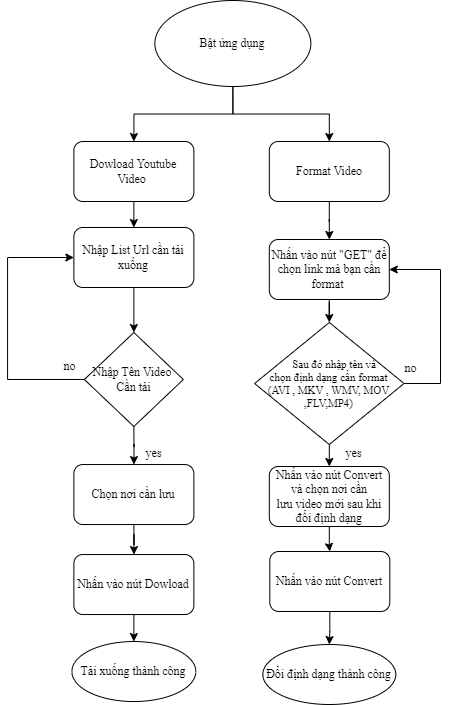
\includegraphics[height=20cm]{images/flowchart.png}
    \caption{Sơ đồ luồng dữ liệu}
    \label{fig:enter-label}
\end{figure}
\newpage

\phantomsection %Tạo điểm cho href nhảy đến cho section*
\section*{Chương 3. KẾT QUẢ ĐẠT ĐƯỢC}
\addcontentsline{toc}{section}{\numberline {}Chương 3.  KẾT QUẢ ĐẠT ĐƯỢC}
\setcounter{section}{3}
\setcounter{subsection}{0}
\subsection{Giao diện chính của ứng dụng}
\begin{figure}[H]
    \centering
    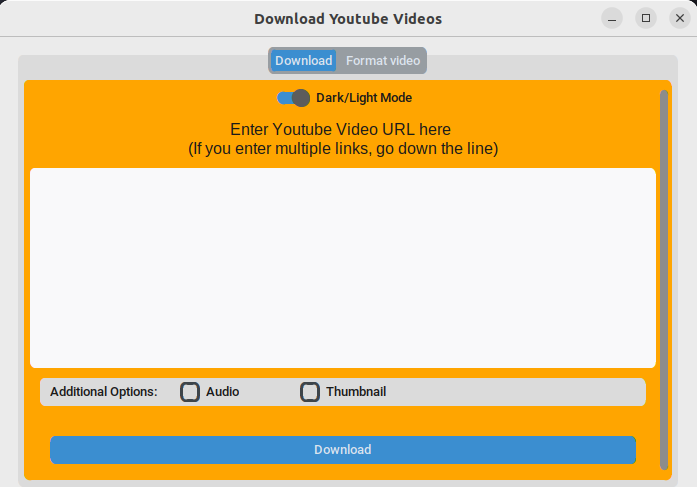
\includegraphics[width=15cm, height=10cm]{images/main1.PNG}
    \caption{Giao diện chính}
    \label{fig:enter-label}
\end{figure}
\begin{figure}[H]
    \centering
    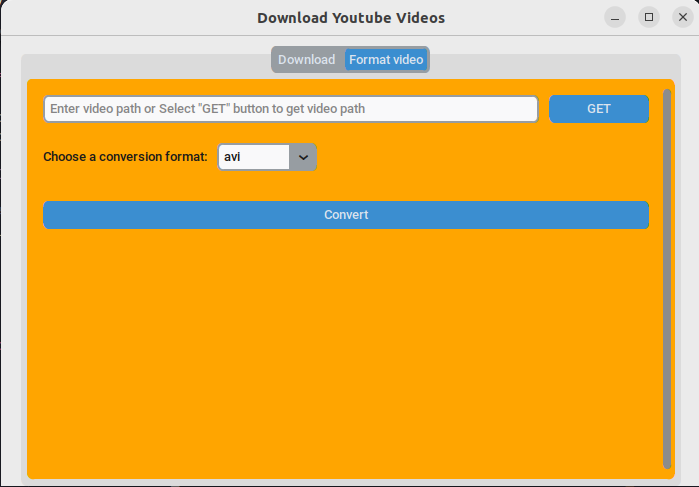
\includegraphics[width=15cm, height=9cm]{images/main2.PNG}
    \caption{Giao diện chuyển đổi định dạng video}
    \label{fig:enter-label}
\end{figure}
\begin{figure}[H]
    \centering
    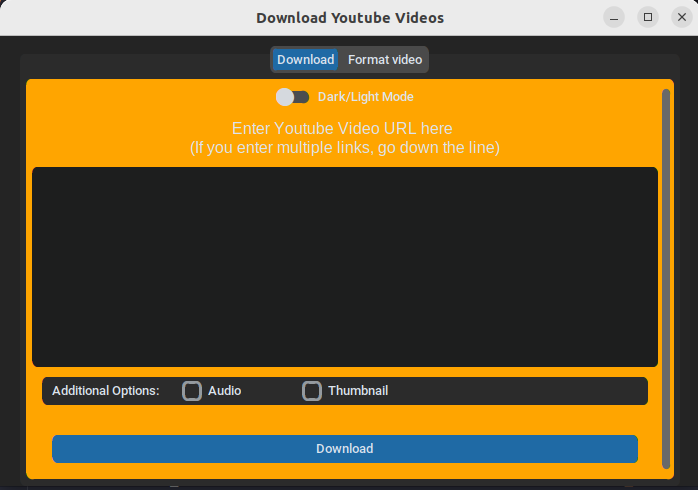
\includegraphics[width=15cm, height=9cm]{images/main3.PNG}
    \caption{Giao diện khi chuyển sang dark mode}
    \label{fig:enter-label}
\end{figure}
\subsection{Tiến hành tải video}
Dán đường link của video muốn tải, sau đó chọn thêm options (nếu có nhu cầu). Tiếp theo, nhấn nút download thì sẽ cho người dùng chọn nơi để lưu thư mục chứa video.
\begin{figure}[H]
    \centering
    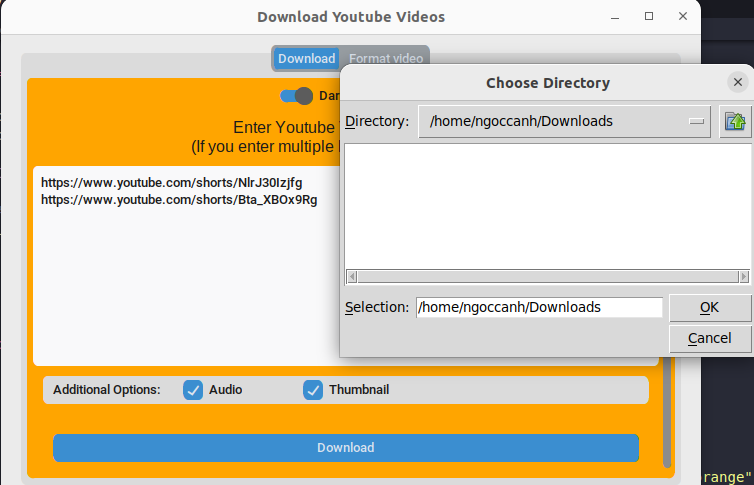
\includegraphics[width=15cm, height=9cm]{images/tienhanh1.PNG}
    \caption{Giao diện chọn vị trí lưu trước khi tải video}
    \label{fig:enter-label}
\end{figure}
\begin{figure}[H]
    \centering
    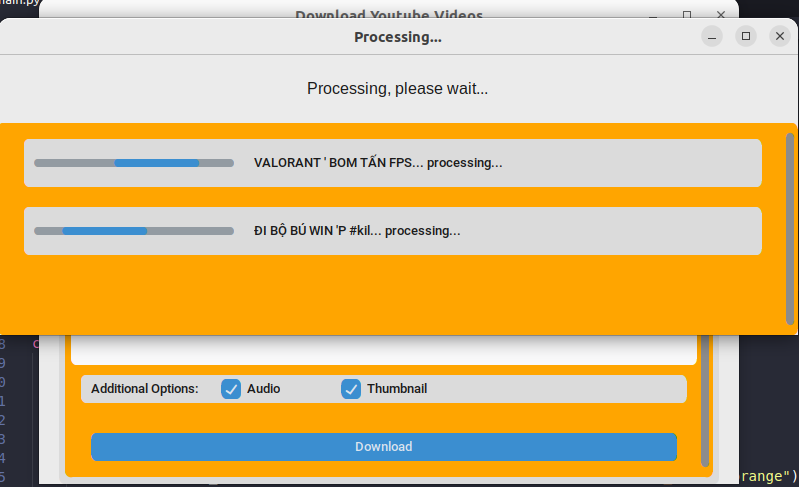
\includegraphics[width=15cm, height=10cm]{images/tienhanh2.PNG}
    \caption{Giao diện đang trong quá trình tải video}
    \label{fig:enter-label}
\end{figure}
\begin{figure}[H]
    \centering
    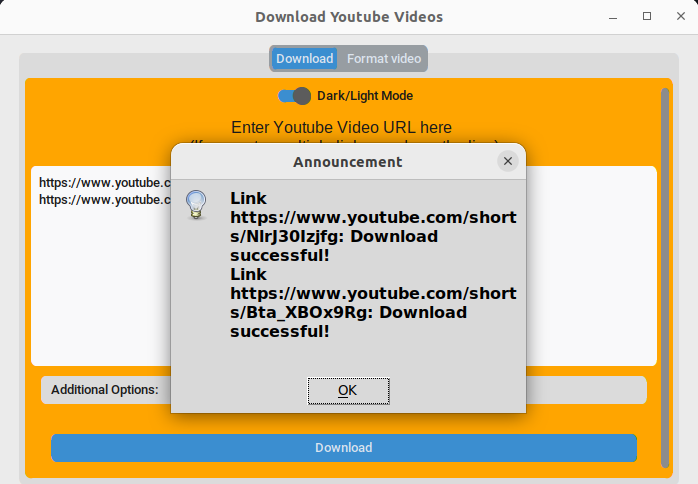
\includegraphics[width=15cm, height=10cm]{images/tienhanh3.PNG}
    \caption{Giao diện khi hoàn thành việc tải video}
    \label{fig:enter-label}
\end{figure}
Cuối cùng hãy vào thư mục đã chọn lúc download để xem kết quả.
\subsection{Tiến hành chuyển đổi định dạng video}
Đầu tiên hãy nhấn nút "GET" để chọn video muốn chuyển đổi định dạng.
\begin{figure}[H]
    \centering
    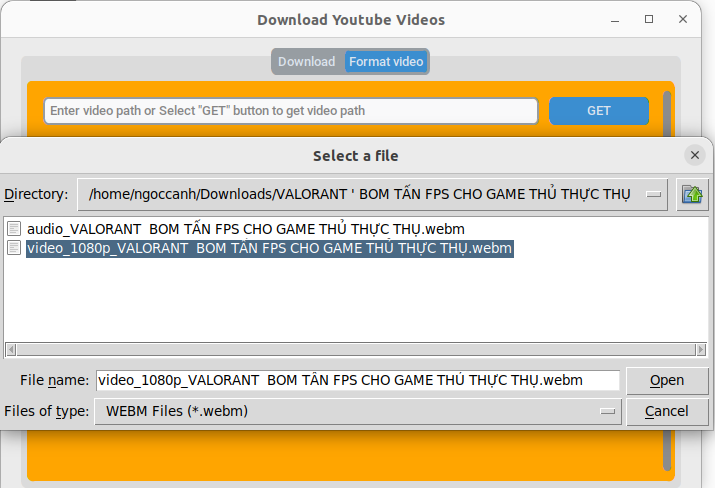
\includegraphics[width=15cm, height=10cm]{images/tienhanh5.PNG}
    \caption{Giao diện chọn video}
    \label{fig:enter-label}
\end{figure}
Tiếp theo là chọn định dạng muốn chuyển.
\begin{figure}[H]
    \centering
    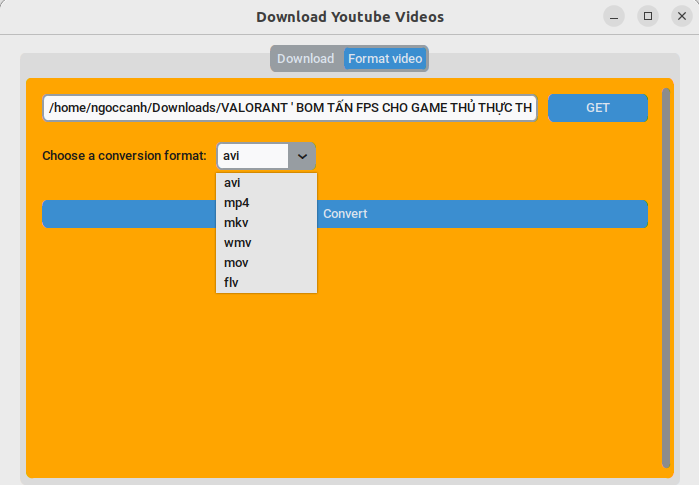
\includegraphics[width=14cm, height=9cm]{images/tienhanh6.PNG}
    \caption{Giao diện chọn định dạng mong muốn cho video}
    \label{fig:enter-label}
\end{figure}
Chọn nơi để lưu khi nhấn nút Convert
\begin{figure}[H]
    \centering
    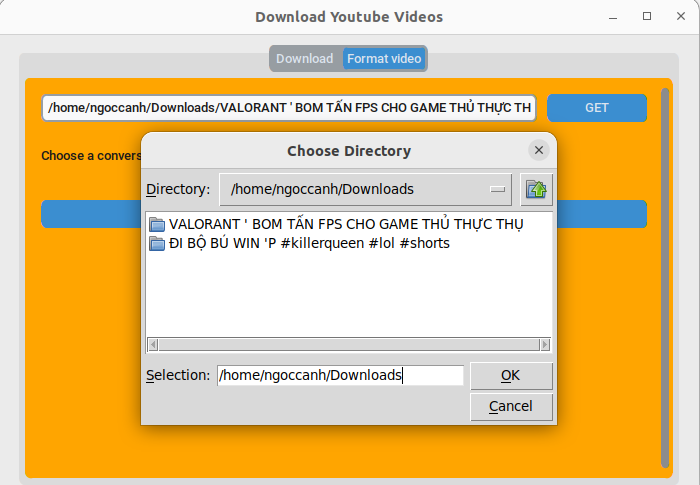
\includegraphics[width=15cm, height=10cm]{images/tienhanh7.PNG}
    \caption{Giao diện chọn nơi để lưu khi nhấn nút convert}
    \label{fig:enter-label}
\end{figure}
\begin{figure}[H]
    \centering
    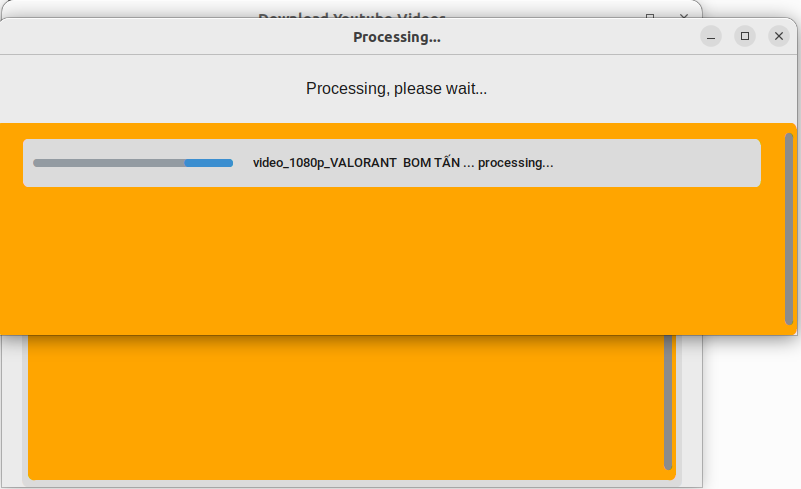
\includegraphics[width=15cm, height=10cm]{images/tienhanh8.PNG}
    \caption{Giao diện đang trong quá trình chuyển đổi định dạng}
    \label{fig:enter-label}
\end{figure}
\begin{figure}[H]
    \centering
    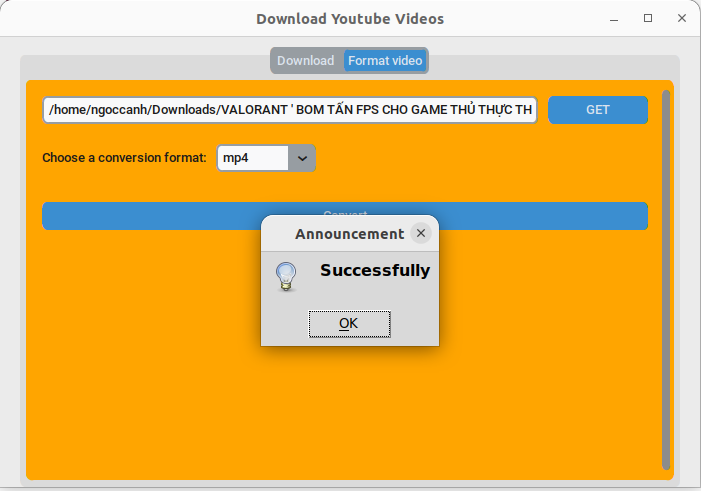
\includegraphics[width=15cm, height=10cm]{images/tienhanh9.PNG}
    \caption{Giao diện khi hoàn thành việc chuyển đổi định dạng video}
    \label{fig:enter-label}
\end{figure}
Cuối cùng hãy vào thư mục đã chọn lúc nảy để xem kết quả.
\newpage

\phantomsection %Tạo điểm cho href nhảy đến cho section*
\section*{Chương 4. CÀI ĐẶT DỰ ÁN}
\addcontentsline{toc}{section}{\numberline {}Chương 4.  CÀI ĐẶT DỰ ÁN}
\setcounter{section}{4}
\setcounter{subsection}{0}
\subsection*{Bước 1: Tải xuống mã nguồn từ github}
Trước tiên, bạn cần tải xuống mã nguồn của dự án từ Github. Bạn có thể truy cập vào trang Github của dự án tại đây: https://github.com/chicong291002/dowload-video
\subsection*{Bước 2: Cài đặt Python cho Linux (nếu chưa có)}
Ứng dụng được viết bằng Python, vì vậy bạn cần cài đặt Python trên máy tính của mình nếu chưa có. Bạn có thể tải xuống phiên bản mới nhất của Python từ trang chủ của Python tại địa chỉ https://www.python.org/downloads/
\subsection*{Bước 3: Cài đặt các thư viện cần thiết}
Mở Command Prompt hoặc Terminal và điều hướng đến thư mục chứa mã nguồn của ứng dụng, sau đó chạy lệnh sau để cài đặt các thư viện cần thiết:
\begin{itemize}
    \item Nếu chưa có pip dùng lệnh sau để cài đặt pip: sudo apt-get update và sudo apt-get install python3-pip
    \item Bạn có thể cài đặt các thư viện cần thiết bằng cách sử dụng file requirements.txt đi kèm với mã nguồn: pip install -r requirements.txt
    \item Tải tkinter: sudo apt-get install python3-tk
    \item Tải ffmpeg: sudo apt-get install ffmpeg
\end{itemize}
\subsection*{Bước 4: Chạy ứng dụng}
Sau khi cài đặt Python và các thư viện cần thiết, bạn có thể chạy ứng dụng bằng cách mở Command Prompt hoặc Terminal và điều hướng đến thư mục chứa mã nguồn của ứng dụng và chạy lệnh sau: python3 main.py
\newpage

\phantomsection %Tạo điểm cho href nhảy đến cho section*
\section*{NHIỆM VỤ, VAI TRÒ CỦA TỪNG THÀNH VIÊN}
\addcontentsline{toc}{section}{\numberline {}NHIỆM VỤ, VAI TRÒ CỦA TỪNG THÀNH VIÊN}
\setcounter{section}{5}
\subsection*{1. Mai Ngọc Cảnh - 3120410064}
\begin{itemize}
    \item Thiết kế giao diện của ứng dụng
    \item Viết báo cáo bằng Latex
\end{itemize}
\subsection*{2. Nguyễn Chí Công - 3120410073}
\begin{itemize}
    \item Xử lý các chức năng trong ứng dụng
    \item Thiết kế giao diện Github
    \item Thiết kế web tĩnh về thông tin phần mềm đang phát triển.
\end{itemize}
\newpage

\phantomsection %Tạo điểm cho href nhảy đến cho section*
\section*{TÀI LIỆU THAM KHẢO}
\addcontentsline{toc}{section}{\numberline {}TÀI LIỆU THAM KHẢO}
\begin{itemize}
    \item[\textbf{[1]}] Thư viện CustomTkinter:  https://github.com/TomSchimansky/CustomTkinter 
    \item[\textbf{[2]}] Thư viện Tkinter: https://www.geeksforgeeks.org/python-gui-tkinter/ 
    \item[\textbf{[3]}] Tổng quan về Python: https://funix.edu.vn/chia-se-kien-thuc/uu-diem-va-nhuoc-diem-cua-python/ 
    \item[\textbf{[4]}] Thư viện Pytube: https://pytube.io/en/latest/index.html 
\end{itemize}
\newpage

\end{document}
